\documentclass{standalone}
\usepackage[dvipsnames,svgnames,x11names]{xcolor}
\usepackage{tikz}
\usetikzlibrary{patterns}
\usepackage{pgfplots}
\pgfplotsset{compat = 1.12}
\usepackage{../thesismath}
\begin{document}
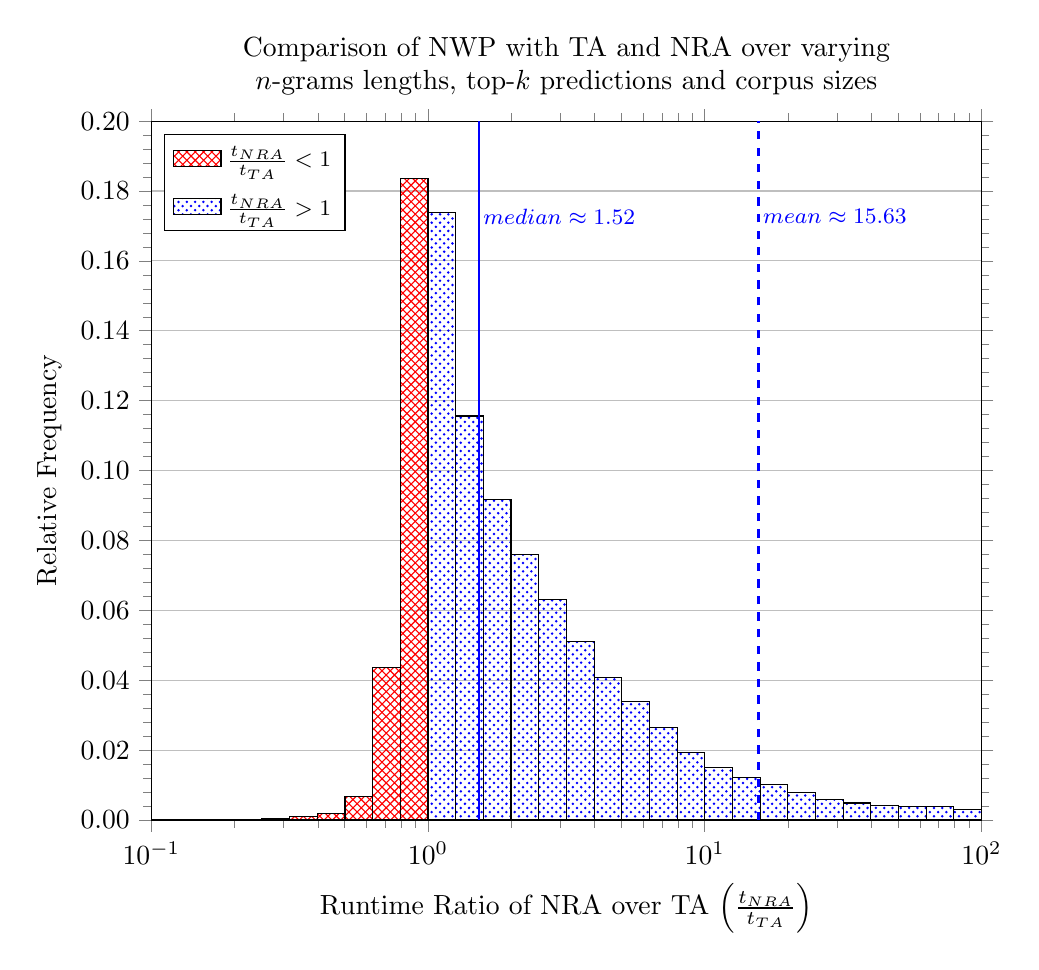
\begin{tikzpicture}[baseline]

\begin{axis}[
  align = center,
  title = {Comparison of NWP with TA and NRA over varying\\$n$-grams lengths, top-$k$ predictions and corpus sizes},
  xlabel = {Runtime Ratio of NRA over TA $\left(\frac{t_\text{NRA}}{t_\text{TA}}\right)$},
  xmode = log,
  xmin = 0.1,
  xmax = 100,
  ylabel = {Relative Frequency},
  ymin = 0,
  ymax = 0.2,
  xtick align = outside,
  ytick align = outside,
  y tick label style = {
    /pgf/number format/fixed,
    /pgf/number format/fixed zerofill,
  },
  minor y tick num = 4,
  ymajorgrids = true,
  legend entries = {{\footnotesize$\frac{t_\text{NRA}}{t_\text{TA}} < 1$},
                    {\footnotesize$\frac{t_\text{NRA}}{t_\text{TA}} > 1$}},
  legend pos = north west,
  legend style = {
    row sep = 1ex,
    xshift = -0.15cm,
    yshift =  0.1cm,
  },
  area legend,
  width = \textwidth,
]

\addplot[
  draw = black,
  pattern = crosshatch,
  pattern color = red,
  ybar interval
] plot coordinates {
  (  0.1       , 2.253787e-05)
  (  0.12589254, 2.864983e-05)
  (  0.15848932, 6.073764e-05)
  (  0.19952623, 1.247859e-04)
  (  0.25118864, 5.331415e-04)
  (  0.31622777, 8.896727e-04)
  (  0.39810717, 1.868224e-03)
  (  0.50118723, 6.792811e-03)
  (  0.63095734, 4.363942e-02)
  (  0.79432823, 1.835270e-01)
  (  1.        , 1.835270e-01)
};
\addplot[
  draw = black,
  pattern = crosshatch dots,
  pattern color = blue,
  ybar interval
] plot coordinates {
  (  1.        , 1.737457e-01)
  (  1.25892541, 1.155962e-01)
  (  1.58489319, 9.162572e-02)
  (  1.99526231, 7.606555e-02)
  (  2.51188643, 6.318370e-02)
  (  3.16227766, 5.119852e-02)
  (  3.98107171, 4.067219e-02)
  (  5.01187234, 3.396100e-02)
  (  6.30957344, 2.651421e-02)
  (  7.94328235, 1.929865e-02)
  ( 10.        , 1.498042e-02)
  ( 12.58925412, 1.207253e-02)
  ( 15.84893192, 1.025524e-02)
  ( 19.95262315, 7.834646e-03)
  ( 25.11886432, 5.825720e-03)
  ( 31.6227766 , 4.877347e-03)
  ( 39.81071706, 4.035679e-03)
  ( 50.11872336, 3.899051e-03)
  ( 63.09573445, 3.808390e-03)
  ( 79.43282347, 3.062603e-03)
  (100.        , 3.062603e-03)
};

\draw [thick, blue]
  ({axis cs:1.52357428016,0}|-{rel axis cs:0,0}) -- ({axis cs:1.52357428016,0}|-{rel axis cs:0,1})
  node [right, xshift = -0.2em, yshift = -0.1\textwidth] {\footnotesize$\text{median} \approx 1.52$};
\draw [thick, blue, dashed]
  ({axis cs:15.6303903973,0}|-{rel axis cs:0,0}) -- ({axis cs:15.6303903973,0}|-{rel axis cs:0,1})
  node [right, xshift = -0.2em, yshift = -0.1\textwidth] {\footnotesize$\text{mean} \approx 15.63$};

\end{axis}

\end{tikzpicture}
\end{document}
